% Options for packages loaded elsewhere
\PassOptionsToPackage{unicode}{hyperref}
\PassOptionsToPackage{hyphens}{url}
%
\documentclass[
  9pt,
  ignorenonframetext,
]{beamer}
\usepackage{pgfpages}
\setbeamertemplate{caption}[numbered]
\setbeamertemplate{caption label separator}{: }
\setbeamercolor{caption name}{fg=normal text.fg}
\beamertemplatenavigationsymbolsempty
% Prevent slide breaks in the middle of a paragraph
\widowpenalties 1 10000
\raggedbottom
\setbeamertemplate{part page}{
  \centering
  \begin{beamercolorbox}[sep=16pt,center]{part title}
    \usebeamerfont{part title}\insertpart\par
  \end{beamercolorbox}
}
\setbeamertemplate{section page}{
  \centering
  \begin{beamercolorbox}[sep=12pt,center]{part title}
    \usebeamerfont{section title}\insertsection\par
  \end{beamercolorbox}
}
\setbeamertemplate{subsection page}{
  \centering
  \begin{beamercolorbox}[sep=8pt,center]{part title}
    \usebeamerfont{subsection title}\insertsubsection\par
  \end{beamercolorbox}
}
\AtBeginPart{
  \frame{\partpage}
}
\AtBeginSection{
  \ifbibliography
  \else
    \frame{\sectionpage}
  \fi
}
\AtBeginSubsection{
  \frame{\subsectionpage}
}
\usepackage{lmodern}
\usepackage{amsmath}
\usepackage{ifxetex,ifluatex}
\ifnum 0\ifxetex 1\fi\ifluatex 1\fi=0 % if pdftex
  \usepackage[T1]{fontenc}
  \usepackage[utf8]{inputenc}
  \usepackage{textcomp} % provide euro and other symbols
  \usepackage{amssymb}
\else % if luatex or xetex
  \usepackage{unicode-math}
  \defaultfontfeatures{Scale=MatchLowercase}
  \defaultfontfeatures[\rmfamily]{Ligatures=TeX,Scale=1}
\fi
\usetheme[]{Goettingen}
\usecolortheme{rose}
% Use upquote if available, for straight quotes in verbatim environments
\IfFileExists{upquote.sty}{\usepackage{upquote}}{}
\IfFileExists{microtype.sty}{% use microtype if available
  \usepackage[]{microtype}
  \UseMicrotypeSet[protrusion]{basicmath} % disable protrusion for tt fonts
}{}
\makeatletter
\@ifundefined{KOMAClassName}{% if non-KOMA class
  \IfFileExists{parskip.sty}{%
    \usepackage{parskip}
  }{% else
    \setlength{\parindent}{0pt}
    \setlength{\parskip}{6pt plus 2pt minus 1pt}}
}{% if KOMA class
  \KOMAoptions{parskip=half}}
\makeatother
\usepackage{xcolor}
\IfFileExists{xurl.sty}{\usepackage{xurl}}{} % add URL line breaks if available
\IfFileExists{bookmark.sty}{\usepackage{bookmark}}{\usepackage{hyperref}}
\hypersetup{
  pdftitle={BIOS6643 Longitudinal},
  pdfauthor={EJC},
  hidelinks,
  pdfcreator={LaTeX via pandoc}}
\urlstyle{same} % disable monospaced font for URLs
\newif\ifbibliography
\setlength{\emergencystretch}{3em} % prevent overfull lines
\providecommand{\tightlist}{%
  \setlength{\itemsep}{0pt}\setlength{\parskip}{0pt}}
\setcounter{secnumdepth}{-\maxdimen} % remove section numbering
\AtBeginSubsection{}
\AtBeginSection{}
\ifluatex
  \usepackage{selnolig}  % disable illegal ligatures
\fi

\title{BIOS6643 Longitudinal}
\subtitle{L9 Softwares}
\author{EJC}
\date{}
\institute{Department of Biostatistics \& Informatics}

\begin{document}
\frame{\titlepage}

\begin{frame}[allowframebreaks]
  \tableofcontents[hideallsubsections]
\end{frame}
\hypertarget{softwares}{%
\section{Softwares}\label{softwares}}

\begin{frame}{Topics for this lecture:}
\protect\hypertarget{topics-for-this-lecture}{}
\begin{itemize}
\item
  A Comparison of SAS versus R for fitting LMMs
\item
  Computation methods for LMMs
\item
  Convergence issues, warnings and unusual estimates in SAS, PROC MIXED
\end{itemize}

\vspace{\baselineskip}

\begin{itemize}
\tightlist
\item
  \textbf{Associated reading: LMM: software and computational issues
  chapter}
\end{itemize}
\end{frame}

\begin{frame}{A Comparison of SAS versus R for fitting LMMs}
\protect\hypertarget{a-comparison-of-sas-versus-r-for-fitting-lmms}{}
There are two common packages with functions that fixed mixed models:
lme4 and nlme. The lme4 package has a function called lmer (stands for
linear mixed-effect regression model). This function will handle many
different types of random effects but does not allow for modeling of
non-simple error covariance structures. However, you can fit generalized
linear mixed models using the glmer function. The nlme package has the
lme function that allows for modeling of both \(\pmb G\) and \(\pmb R\)
matrices , although it cannot handle some more complex models very
easily.

In this section we first look at a crossed random effect model using the
lmer function from lme4, and then consider different covariance modeling
approaches using the lme function.
\end{frame}

\begin{frame}{Rater and subject data and the lmer function}
\protect\hypertarget{rater-and-subject-data-and-the-lmer-function}{}
These data were first presented in the LMM intro notes, where 4 judges
(or raters) each rated 6 subjects. In one model we used subject and
rater as crossed random effects. Here was the model (called `Approach 1'
in previous notes.)

\(Y_{ij}=\mu +b_{iS}+b_{jR}+\epsilon_{ij}\), where \(i\) denotes subject
and \(j\) denotes judge;

\(b_{iS} \sim \mathcal N(0,\  \sigma_S^2),\ b_{jR} \sim \mathcal N(0,\  \sigma_R^2),\ \epsilon_{ij} \sim \mathcal N(0,\  \sigma_\epsilon^2)\),
all independent.
\end{frame}

\begin{frame}{}
\protect\hypertarget{section}{}
Below is the SAS approach on the left, with the equivalent R approach on
the right.

\begin{center}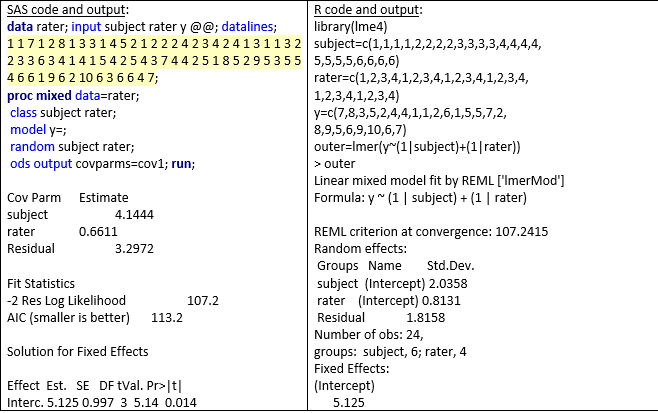
\includegraphics[width=0.7\linewidth]{figs_L9/f1} \end{center}
\end{frame}

\begin{frame}{Dental data and the lme function}
\protect\hypertarget{dental-data-and-the-lme-function}{}
\begin{block}{Examples employ the lme function within the nlme package.}
\protect\hypertarget{examples-employ-the-lme-function-within-the-nlme-package.}{}
Data set: sample data from R, Orthodont (included with package nlme).
Four variables: DISTANCE, AGE, SUBJECT, SEX. There are 4 measures on 27
subjects, at ages 8, 10, 12 and 14. The primary outcome is DISTANCE. The
data is in `data.frame' form.

Estimation method used here: REML.
\end{block}

\begin{block}{Computational methods:}
\protect\hypertarget{computational-methods}{}
SAS generally uses Newton-Raphson Ridge regression. R states ``The
computational methods follow on the general framework of Lindstrom and
Bates (1988), JASA, Newton-Raphson and EM Algorithms for Linear
Mixed-Effects Models for Repeated-Measures Data.''
\end{block}
\end{frame}

\begin{frame}{Degrees of freedom:}
\protect\hypertarget{degrees-of-freedom}{}
The method for selecting denominator degrees of freedom in SAS depends
on whether a RANDOM or REPEATED (or both) are included.

\begin{itemize}
\item
  For the given data and code, if there is a RANDOM statement, the
  `containment' method is used (whether or not a REPEATED statement is
  used.
\item
  If there is a REPEATED but no RANDOM statement, then the
  `between-within' method is used.
\item
  The DDFM option in the MODEL statement can be used to specify the DDF
  method, there are about 5 to choose from.
\end{itemize}
\end{frame}

\begin{frame}{There is no mention in R about DDF}
\protect\hypertarget{there-is-no-mention-in-r-about-ddf}{}
For the fixed effects other than intercept, the DDF appears to be like
that of the `between-within' method for the LME function.

The intercept DDF is different than that of any method in SAS.

For the GLS function, R appears to use the `residual' method for DDF
(since you get the same p-values in SAS when you specify DDFM=residual
for Model II, and the Residual DDF is mentioned at the end of the R
output).
\end{frame}

\begin{frame}{}
\protect\hypertarget{section-1}{}
Three models fit:

\begin{itemize}
\item
  random intercept only
\item
  AR(1) structure only
\item
  random intercept plus AR(1).
\end{itemize}

For models using random terms, the lme function can be used; for those
without random terms but a specified R matrix (such as AR(1)), the gls
function (generalized least squares) will fit the model.
\end{frame}

\begin{frame}{Model I}
\protect\hypertarget{model-i}{}
\begin{center}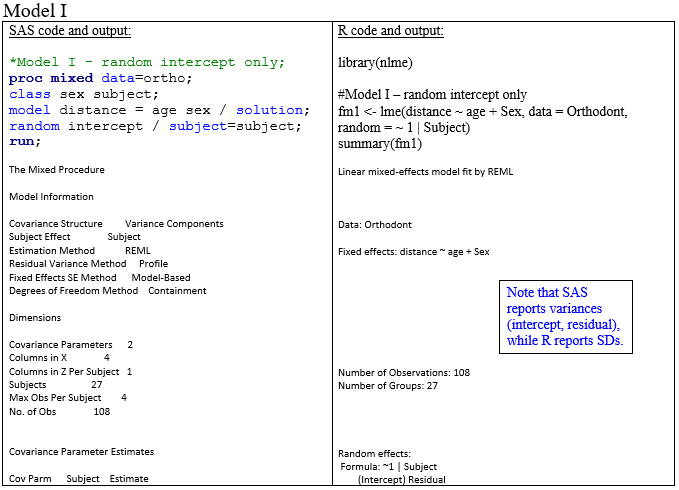
\includegraphics[width=0.7\linewidth]{figs_L9/f2} \end{center}

\begin{center}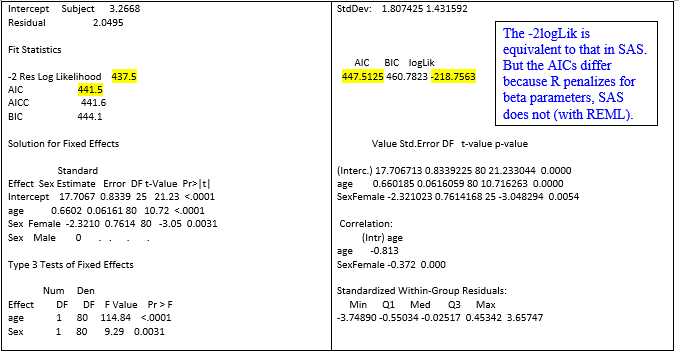
\includegraphics[width=0.7\linewidth]{figs_L9/f3} \end{center}
\end{frame}

\begin{frame}{Model II}
\protect\hypertarget{model-ii}{}
\begin{center}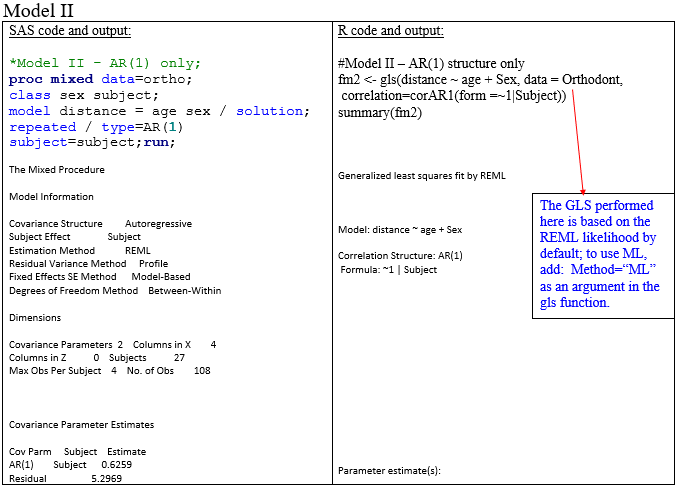
\includegraphics[width=0.7\linewidth]{figs_L9/f4} \end{center}

\begin{center}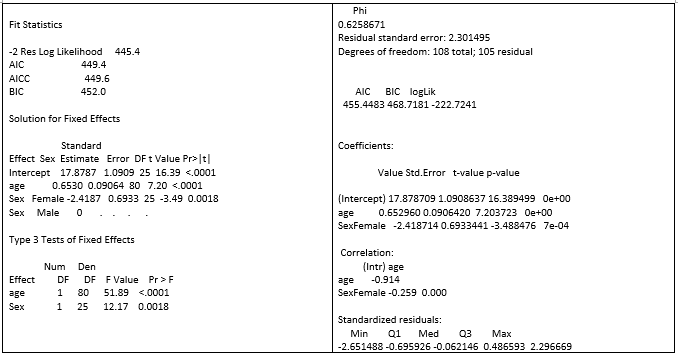
\includegraphics[width=0.7\linewidth]{figs_L9/f5} \end{center}
\end{frame}

\begin{frame}{Model III}
\protect\hypertarget{model-iii}{}
\begin{center}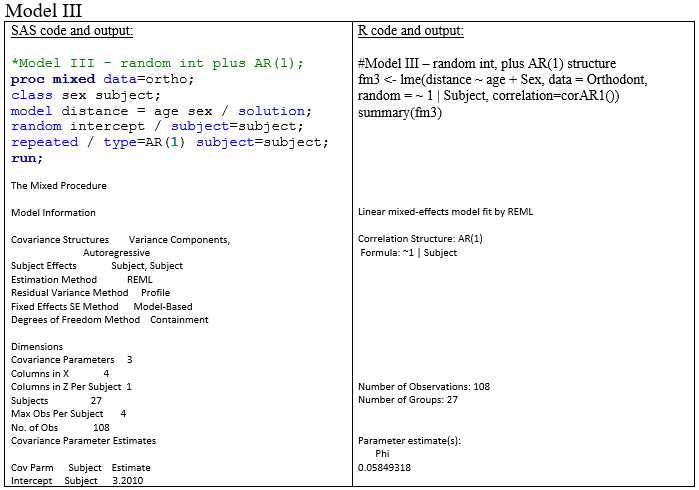
\includegraphics[width=0.7\linewidth]{figs_L9/f6} \end{center}

\begin{center}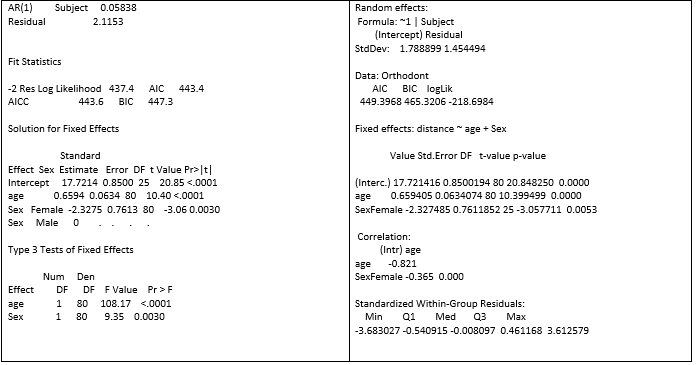
\includegraphics[width=0.7\linewidth]{figs_L9/f7} \end{center}
\end{frame}

\hypertarget{more-detail-regarding-computational-methods-for-lmm}{%
\section{More detail regarding computational methods for
LMM}\label{more-detail-regarding-computational-methods-for-lmm}}

\begin{frame}{Starting values for alpha parameters}
\protect\hypertarget{starting-values-for-alpha-parameters}{}
For a numerical technique such as Newton-Raphson Ridge regression (which
SAS uses in PROC MIXED), you need starting values for the
\(\pmb \alpha\) parameters.

You can either specify these starting values using the PARMS statement
in PROC MIXED, or use the default, which is to use the MIVQUE0 estimator
values. MIVQUE0 is actually a method that can be specified as an
estimation method in the PROC MIXED statement (PROC MIXED
METHOD=MIVQUE0;). This is typically not done.

MIVQUE0 performs minimum variance quadratic unbiased estimation of the
covariance parameters, which is a form of method of moments estimation,
and it does not require an iterative method. However, simulations have
shown that REML and ML are more accurate.

Nevertheless, since MIVQUE0 is based on algebraic forms and does not
rely on numerical analysis, it may be useful for extremely large data
sets.
\end{frame}

\begin{frame}{Algorithms to perform ML, REML estimation}
\protect\hypertarget{algorithms-to-perform-ml-reml-estimation}{}
In fitting an LMM, we discussed how a ridge-stabilized Newton-Raphson
algorithm is commonly used (e.g., in SAS) to maximize the likelihood
with respect to the \(\pmb \alpha\) parameters. (Estimates of
\(\pmb \beta\) can then be found in closed form.)

There are other computational methods that can be used to fit an LMM,
including the expectation maximization (EM) algorithm, or Fisher's
Scoring method.

The EM algorithm may be useful in fitting more complex LMMs such as
\textbf{heterogeneity models} that allow for random terms that have
non-normal distributions. {[}The non-normal distributions can be
constructed using a mixture of normals (see Verbeke, 2000).{]}
\end{frame}

\begin{frame}{}
\protect\hypertarget{section-2}{}
The NR algorithm may not yield convergence for such models due to their
complexity. The EM algorithm, which is particularly useful for ML
estimation when missing data are involved. The ``E step'' is the
expectation step; the ``M step'' is the maximization step. The basic
steps of the EM algorithm are as follows.

\begin{enumerate}
\item
  Obtain starting values of the parameters, call it \(\theta^{(1)}\).
\item
  \emph{The E step}: Let \(y^0\) denote the observed data and let
  \(\theta^{(t)}\) denote the current value of the parameter vector
  theta (t=1 the first time through). Determine
  \(E[L(\theta |y)\ |\ y^0,\ \theta ^{(t)}]\)
\item
  \emph{The M step}: Determine \(\pmb \theta^{(t)}\) that maximizes
  \(E[L(\theta |y)\ |\ y^0,\ \theta ^{(t)}]\).
\item
  Repeat steps (ii) and (iii) until convergence.
\end{enumerate}
\end{frame}

\begin{frame}{}
\protect\hypertarget{section-3}{}
The EM algorithm typically has a slow rate of convergence. Also, it is
more likely to converge at a local maximum instead of global, making
precision of estimates more uncertain.

It is for these reasons that the Newton-Raphson or Fisher Scoring
algorithms are preferred. On the other hand, direct likelihood
maximization techniques may have convergence problems for more complex
models. In such cases, the EM can be considered.

While the NR algorithm uses the Hessian or observed information matrix
(the matrix of second-order derivatives of the log-likelihood function),
Fisher's Scoring method uses the expected information matrix, or
expected Hessian matrix.

It is possible to start the numerical optimization using Fisher's
Scoring method for a certain number of iterations, and then switch over
to the NR method.
\end{frame}

\begin{frame}{}
\protect\hypertarget{section-4}{}
In PROC MIXED, including SCORING\textless=number\textgreater{} will tell
SAS to use Fisher's Scoring Method up to the specified number, after
which the NR algorithm will be used. For more detail, see Verbeke (2000)
and the SAS Help Documentation.

Some other facts about Fisher's Scoring Method

\begin{itemize}
\item
  Yields equivalent results as `Iteratively Reweighted Least Squares'.
\item
  Often used to maximize Generalized linear model (GzLM) likelihoods,
  although the default in PROC GENMOD is once again the NR algorithm
  (see SAS Help Documentation).
\end{itemize}

For more use of NR, EM or Fisher's Scoring method to achieve numerical
ML or REML estimates, see Verbeke (2000).
\end{frame}

\hypertarget{convergence-issues-warnings-and-unusual-estimates-in-sas-proc-mixed}{%
\section{Convergence issues, warnings and unusual estimates in SAS, PROC
MIXED}\label{convergence-issues-warnings-and-unusual-estimates-in-sas-proc-mixed}}

\begin{frame}{Introduction}
\protect\hypertarget{introduction}{}
Sometimes when fitting a linear mixed model with data you will have
convergence issues. That is, the iterative numerical method used to
maximize the likelihood or restricted likelihood fails to meet
convergence criteria so that estimates cannot be obtained.

In other cases, you may get estimates or a partial set of estimates but
you will get a warning that a problem occurred, such as a `non-positive
definite' matrix.

Some of the convergence problems are discussed in these notes. Here, I
focus on PROC MIXED, although many of the same issues will face other
software that you use to fit LMMs.
\end{frame}

\begin{frame}{Fail-to-converge issues}
\protect\hypertarget{fail-to-converge-issues}{}
SAS Help Documentation indicates that some reasons for non-convergence
of the Newton-Raphson algorithm include flat or ridged likelihood
surfaces, model misspecification or a violation of the normality
assumption.

From my experiences, most of the non-convergence issues that I have run
into are alleviated once I simplify the model a bit, and thus I
generally attribute it to model specification.

If you do have extremely non-normal data, then you really should deal
with that up front by either transforming the data so that it is more
normally distributed (if possible), using a model suitable for the
distribution, or identifying outliers that may be causing problems and
run analyses without them. (However, I am not encouraging you to just
drop the data altogether.
\end{frame}

\begin{frame}{}
\protect\hypertarget{section-5}{}
Ideally, if the points are real, then you want to perform analyses with
and without the points; but if the model cannot handle the points, then
some type of adjust may need to be made in order to perform analyses
`with them'. Or, at the very least, report the values that you were not
able to fit.)

SAS states that ``It is also possible for PROC MIXED to converge to a
point that is not the global optimum of the likelihood, although this
usually occurs only with the spatial covariance structures.''

SAS lists several steps that can be taken in order to try to get the
model to converge if at first you do not succeed. Many of these steps
include specifying options in the optimization routine. For more
details, see `Convergence Problems' within the `Computational Issues'
page in the MIXED documentation.
\end{frame}

\begin{frame}{Unusual estimates for covariance parameters}
\protect\hypertarget{unusual-estimates-for-covariance-parameters}{}
We know that variances should be non-negative, and that correlations
should be between -1 and +1. The optimization routines that carry out
likelihood maximization in PROC MIXED employ these constraints.

It is not that uncommon to see a variance estimate of 0. In terms of
numerical quantities, the actual estimate would be 0 or even negative,
but since there is a constraint that the variance must be nonnegative,
the estimate is 0.

In practical terms, I take this to mean that based on the specified
model, there is no detectable variance for the associated random effect.
Note, however, that it is possible that the variance for the same random
effect is positive (but not necessarily significant) if other parts of
the model are changed. That's why it is important to interpret effects
in relation to the model as a whole.
\end{frame}

\begin{frame}{}
\protect\hypertarget{section-6}{}
By default, covariance parameters are constrained in PROC MIXED
optimization. Variances are not allowed to be negative, and correlations
cannot have an absolute value that exceeds 1.

When you do obtain a covariance parameter estimate that is on the
boundary, it suggests that the estimate using unconstrained optimization
would be out-of-bounds.

For example, using the fitting an AR(1) structure for subjects as well
as including a random intercept for the Ramus data yields an estimate of
0 for the variance associated with the random intercept. If you then
include the NOBOUND option in the PROC MIXED statement (no slash between
them), the variance estimate is a small negative number.

However, note that doing an unconstrained optimization and then setting
the violating estimate to 0 will yield different estimates for other
parameters in the model, relative to the constrained optimization.
\end{frame}

\begin{frame}{Non-positive definite matrices}
\protect\hypertarget{non-positive-definite-matrices}{}
A matrix \(\pmb M\) is positive definite is for any \(1 \times n\)
real-valued vector \(\pmb z\), \(\pmb {zMz}^{\top} > 0\), and \(\pmb M\)
is symmetric. By definition, covariance matrices are required to be
positive definite. However, when fitting models, sometimes this
requirement is not attained, which will either yield a warning, error or
`note' message.

A message that \(\pmb G\) is not positive definite often occurs when a
variance parameter is estimated to be 0. If the associated random effect
term is removed from the model or the model is simplified in some way,
then the message is likely to go away. Although having a non-positive
definite fitted \(\pmb G\) is not desirable, we should keep in mind that
our ultimate goal is to have a realistic fitted \(\pmb V\) matrix.
\end{frame}

\begin{frame}{}
\protect\hypertarget{section-7}{}
Recent runs with \textbf{SAS (v9.3)} on some of my data have only given
me a `note' that \(\pmb G\) was not positive definite, and essentially
removed this parameter from the model as it was not penalized for in the
AIC. In addition, the fitted \(\pmb V\) matrices did seem reasonable.
Thus, if direct interpretation or inference related to this parameter
are not needed and the covariance structure is essentially done to
account to properly handle the correlated data, then using the model
with a `0' variance in \(\pmb G\) may be of practical use. Still, I
would probably search for a decent comparable model for which all
covariance parameters met model assumptions.

You may see a warning or error when the Hessian matrix (matrix of 2nd
order derivatives of the log likelihood function), \(\pmb R\) matrix or
\(\pmb V\) matrix is non-positive-definite. This might occur if there
are problems with the data, such as accidentally having multiple records
for a subject for the same time of measurement.
\end{frame}

\begin{frame}{}
\protect\hypertarget{section-8}{}
Direct quote from SAS Help Documentation: ``An infinite likelihood
during the iteration process means that the Newton-Raphson algorithm has
stepped into a region where either the \(\pmb R\) or \(\pmb V\) matrix
is nonpositive definite. This is usually no cause for concern as long as
iterations continue. If PROC MIXED stops because of an infinite
likelihood, recheck your model to make sure that no observations from
the same subject are producing identical rows in \(\pmb R\) or
\(\pmb V\) and that you have enough data to estimate the particular
covariance structure you have selected. Any time that the final
estimated likelihood is infinite, subsequent results should be
interpreted with caution.''

SAS also states that non-positive definite Hessian matrices can occur
with surface saddlepoints or linear dependencies among the parameters.
\end{frame}

\end{document}
